\documentclass[conference]{IEEEtran}
\IEEEoverridecommandlockouts
% The preceding line is only needed to identify funding in the first footnote. If that is unneeded, please comment it out.
\usepackage{cite}
\usepackage{amsmath,amssymb,amsfonts}
\usepackage{algorithmic}
\usepackage{graphicx}
\usepackage{textcomp}
\usepackage{xcolor}
\def\BibTeX{{\rm B\kern-.05em{\sc i\kern-.025em b}\kern-.08em
    T\kern-.1667em\lower.7ex\hbox{E}\kern-.125emX}}
\begin{document}

\title{Modeling and simulation of Power Consumption on Heterogenous CPU Cores under varying workloads and operating conditions\\

}

\author{\IEEEauthorblockN{Atharv Arun Desai}
\IEEEauthorblockA{\textit{Department of CSA} \\
\textit{Indian Institute of Science (IISc)}\\
Bangalore, India\\
atharvarun@iisc.ac.in}
\and
\IEEEauthorblockN{Boul Chandra Garai}
\IEEEauthorblockA{\textit{Department of CSA} \\
\textit{Indian Institute of Science (IISc)}\\
Bangalore, India \\
chandraboul@iisc.ac.in}
\and
\IEEEauthorblockN{Himanshu Srivastava}
\IEEEauthorblockA{\textit{Department of CSA} \\
\textit{Indian Institute of Science (IISc)}\\
Bangalore, India\\
himanshusriv@iisc.ac.in}
\and
\IEEEauthorblockN{Vaisakh P S}
\IEEEauthorblockA{\textit{Department of CSA} \\
\textit{Indian Institute of Science (IISc)}\\
Bangalore, India\\
vaisakhp@iisc.ac.in}
}

\maketitle

\begin{abstract}
    This document serves as phase-1 report for E0-240 - Modeling and Simulation course project delivery. The main objective of this project is to apply concepts learned in E0-240 course in to Modeling and simulation of a real-world system, which in this case is Multi-core, Heterogenous CPU. This project, will focus on developing a Power Consumption Model for simulated Full-System \cite{8718630} under varying workloads. This model will be developed taking in consideration various operating conditions of the CPU such as Dynamic Frequency Scaling, Heterogenous Cores \cite{arm-big.little-whitepaper}
\end{abstract}

\begin{IEEEkeywords}
    Modeling, simulation, heterogenous CPU cores, power consumption
\end{IEEEkeywords}

\section{Background}


\section{Data Gathering}
    \par test


\section{Phase-2 Observations and Results}
    \par test

\section{Discussion on Phase-2 outcomes}

\section{Next Step}

\begin{figure}[b]
    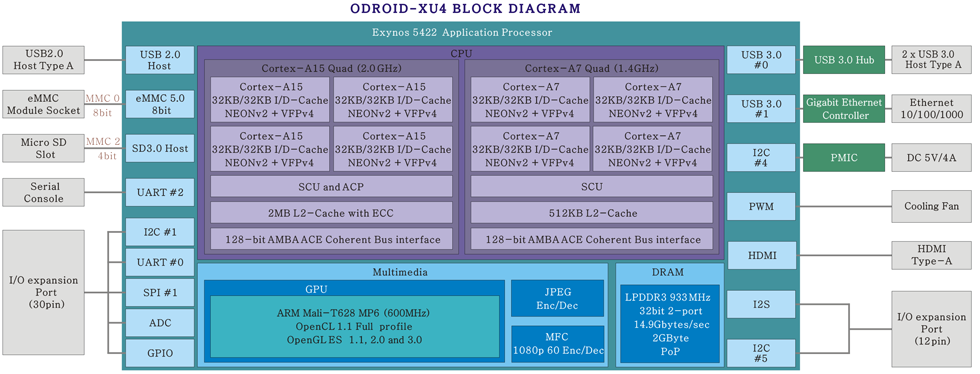
\includegraphics{rsrc/201506191222574523.png}
    \caption{ODroid XU4 board overview}
    \label{fig-odroid-hwoverview}
\end{figure}


\begin{figure}[t]
    \centering
    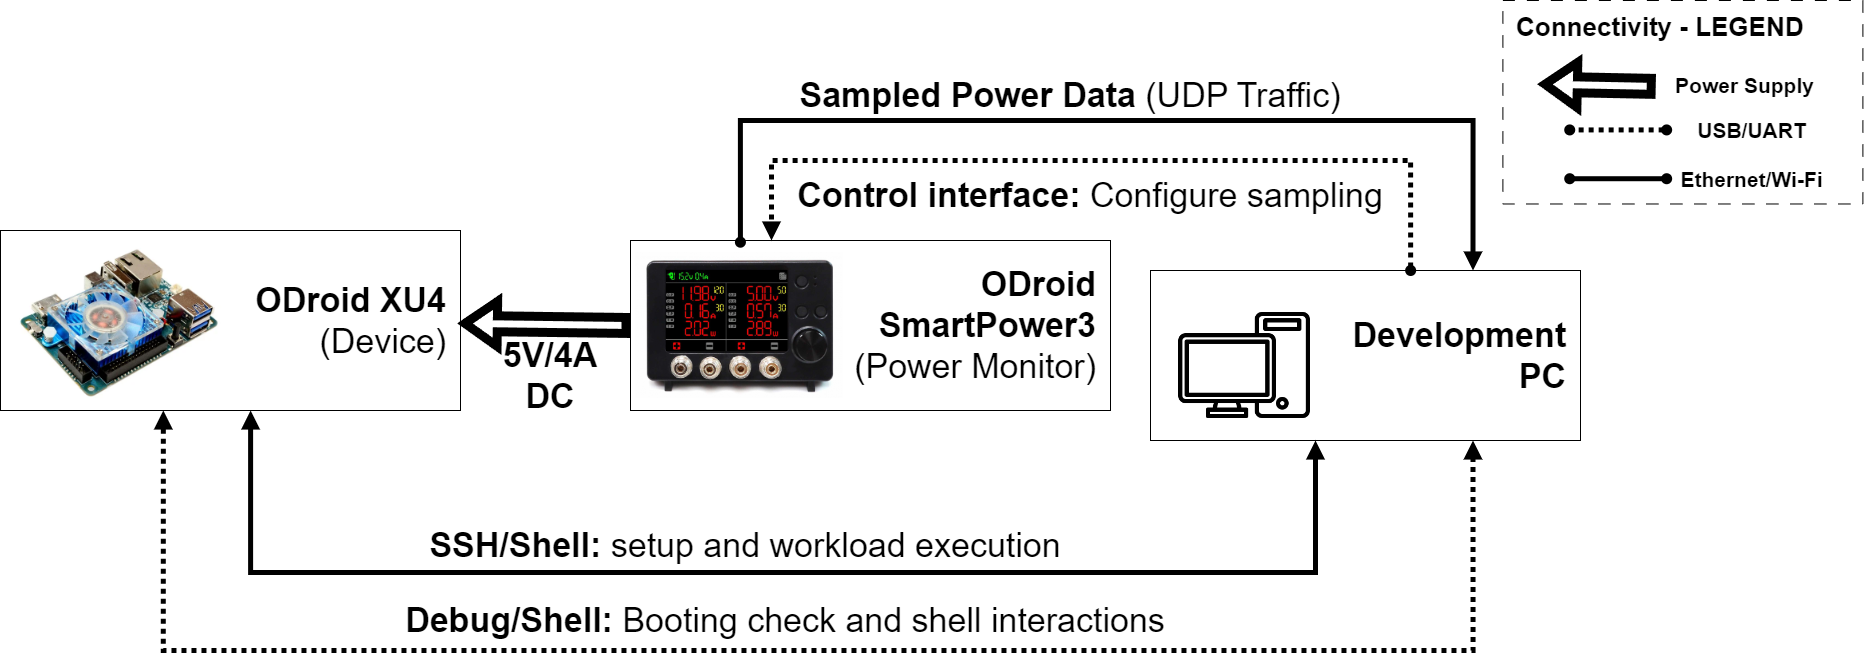
\includegraphics[width=0.48\textwidth]{rsrc/Experiment-setup.drawio.png}
    \caption{Experiment setup for power data gathering from actual hardware}
    \label{fig-Experiment-setup}
\end{figure}


\begin{table}[htbp]
    \caption{List of workloads being used for data gathering and validation}
    \begin{center}
        \begin{tabular}{|c|p{4cm}|c|}
            \hline
            \textbf{Workload}&\multicolumn{2}{|c|}{\textbf{Workload Details}} \\
            \cline{2-3} 
            \textbf{Type} & \multicolumn{1}{|c|}{\textbf{\textit Workloads}} & \textbf{\textit{Status}} \\
            \hline
            Stress Test & stress command \cite{linux-stress-testing} & $\checkmark$ \\
            \hline
            Video Encoding & ffmpeg encode [x] & $\checkmark$ \\
            \hline
            File Compression & gzip, bzip2, xz compression on datasets [x] & $\checkmark$ \\
            \hline
            Benchmark Suite & SPEC2017 [x] & Planned \\
            \hline
        \end{tabular}
        \label{tab1}
    \end{center}
\end{table}
% ------------------------------------------------------------------------------
% Reference and Cited Works
% ------------------------------------------------------------------------------
\newpage
\bibliographystyle{IEEEtran}
\bibliography{references.bib}

% ------------------------------------------------------------------------------

\end{document}
